%%
%% This is file `sample-acmsmall-conf.tex',
%% generated with the docstrip utility.
%%
%% The original source files were:
%%
%% samples.dtx  (with options: `acmsmall-conf')
%% 
%% IMPORTANT NOTICE:
%% 
%% For the copyright see the source file.
%% 
%% Any modified versions of this file must be renamed
%% with new filenames distinct from sample-acmsmall-conf.tex.
%% 
%% For distribution of the original source see the terms
%% for copying and modification in the file samples.dtx.
%% 
%% This generated file may be distributed as long as the
%% original source files, as listed above, are part of the
%% same distribution. (The sources need not necessarily be
%% in the same archive or directory.)
%%
%%
%% Commands for TeXCount
%TC:macro \cite [option:text,text]
%TC:macro \citep [option:text,text]
%TC:macro \citet [option:text,text]
%TC:envir table 0 1
%TC:envir table* 0 1
%TC:envir tabular [ignore] word
%TC:envir displaymath 0 word
%TC:envir math 0 word
%TC:envir comment 0 0
%%
%%
%% The first command in your LaTeX source must be the \documentclass
%% command.
%%
%% For submission and review of your manuscript please change the
%% command to \documentclass[manuscript, screen, review]{acmart}.
%%
%% When submitting camera ready or to TAPS, please change the command
%% to \documentclass[sigconf]{acmart} or whichever template is required
%% for your publication.
%%
%%
\documentclass[acmsmall,anonymous]{acmart}

%%
%% \BibTeX command to typeset BibTeX logo in the docs
\AtBeginDocument{%
  \providecommand\BibTeX{{%
    Bib\TeX}}}

%% Rights management information.  This information is sent to you
%% when you complete the rights form.  These commands have SAMPLE
%% values in them; it is your responsibility as an author to replace
%% the commands and values with those provided to you when you
%% complete the rights form.
\setcopyright{rightsretained}
\copyrightyear{2024}
\acmYear{2024}
\acmDOI{XXXXXXX.XXXXXXX}

%% These commands are for a PROCEEDINGS abstract or paper.
\acmConference[ICFP '24]{International Conference on Functional Programming}{September 02--07,
  2024}{Milan, IT}
%%
%%  Uncomment \acmBooktitle if the title of the proceedings is different
%%  from ``Proceedings of ...''!
%%
%%\acmBooktitle{Woodstock '18: ACM Symposium on Neural Gaze Detection,
%%  June 03--05, 2018, Woodstock, NY}
\acmISBN{978-1-4503-XXXX-X/18/06}


%%
%% Submission ID.
%% Use this when submitting an article to a sponsored event. You'll
%% receive a unique submission ID from the organizers
%% of the event, and this ID should be used as the parameter to this command.
%%\acmSubmissionID{123-A56-BU3}

%%
%% For managing citations, it is recommended to use bibliography
%% files in BibTeX format.
%%
%% You can then either use BibTeX with the ACM-Reference-Format style,
%% or BibLaTeX with the acmnumeric or acmauthoryear sytles, that include
%% support for advanced citation of software artefact from the
%% biblatex-software package, also separately available on CTAN.
%%
%% Look at the sample-*-biblatex.tex files for templates showcasing
%% the biblatex styles.
%%

%%
%% The majority of ACM publications use numbered citations and
%% references.  The command \citestyle{authoryear} switches to the
%% "author year" style.
%%
%% If you are preparing content for an event
%% sponsored by ACM SIGGRAPH, you must use the "author year" style of
%% citations and references.
%% Uncommenting
%% the next command will enable that style.
%%\citestyle{acmauthoryear}

\usepackage{xcolor}
\usepackage{color}
\usepackage{fancyvrb}
\usepackage{framed}

%%
%% end of the preamble, start of the body of the document source.
\begin{document}

%%
%% The "title" command has an optional parameter,
%% allowing the author to define a "short title" to be used in page headers.
\title[TidalCycles: Continuous and Discrete Patterns of FRP]{TidalCycles: Continuous and Discrete Patterns of Functional Reactive Programming}

%%
%% The "author" command and its associated commands are used to define
%% the authors and their affiliations.
%% Of note is the shared affiliation of the first two authors, and the
%% "authornote" and "authornotemark" commands
%% used to denote shared contribution to the research.
\author{Alex McLean}
\authornotemark[1]
\email{alex@slab.org}
\affiliation{%
  \institution{Then Try This}
  \streetaddress{Studio F4, Cuthbert House, Arley Street}
  \city{Sheffield}
  \state{South Yorkshire}
  \country{UK}
  \postcode{S7 2EN}
}

%%
%% By default, the full list of authors will be used in the page
%% headers. Often, this list is too long, and will overlap
%% other information printed in the page headers. This command allows
%% the author to define a more concise list
%% of authors' names for this purpose.
%% \renewcommand{\shortauthors}{Trovato et al.}

%%
%% The abstract is a short summary of the work to be presented in the
%% article.
\begin{abstract}
  Abstract goes here.
\end{abstract}

%%
%% The code below is generated by the tool at http://dl.acm.org/ccs.cfm.
%% Please copy and paste the code instead of the example below.
%%
\begin{CCSXML}
<ccs2012>
   <concept>
       <concept_id>10010405.10010469.10010471</concept_id>
       <concept_desc>Applied computing~Performing arts</concept_desc>
       <concept_significance>500</concept_significance>
       </concept>
   <concept>
       <concept_id>10010405.10010469.10010475</concept_id>
       <concept_desc>Applied computing~Sound and music computing</concept_desc>
       <concept_significance>500</concept_significance>
       </concept>
   <concept>
       <concept_id>10003752.10003753</concept_id>
       <concept_desc>Theory of computation~Models of computation</concept_desc>
       <concept_significance>500</concept_significance>
       </concept>
   <concept>
       <concept_id>10011007.10011006.10011050.10011017</concept_id>
       <concept_desc>Software and its engineering~Domain specific languages</concept_desc>
       <concept_significance>500</concept_significance>
       </concept>
   <concept>
       <concept_id>10011007.10011006.10011008.10011009.10011012</concept_id>
       <concept_desc>Software and its engineering~Functional languages</concept_desc>
       <concept_significance>500</concept_significance>
       </concept>
 </ccs2012>
\end{CCSXML}

\ccsdesc[500]{Applied computing~Performing arts}
\ccsdesc[500]{Applied computing~Sound and music computing}
\ccsdesc[500]{Theory of computation~Models of computation}
\ccsdesc[500]{Software and its engineering~Domain specific languages}
\ccsdesc[500]{Software and its engineering~Functional languages}

%%
%% Keywords. The author(s) should pick words that accurately describe
%% the work being presented. Separate the keywords with commas.
\keywords{pure functional reactive programming, FRP, music representation, algorithmic pattern}
%% A "teaser" image appears between the author and affiliation
%% information and the body of the document, and typically spans the
%% page.
% \begin{teaserfigure}
%  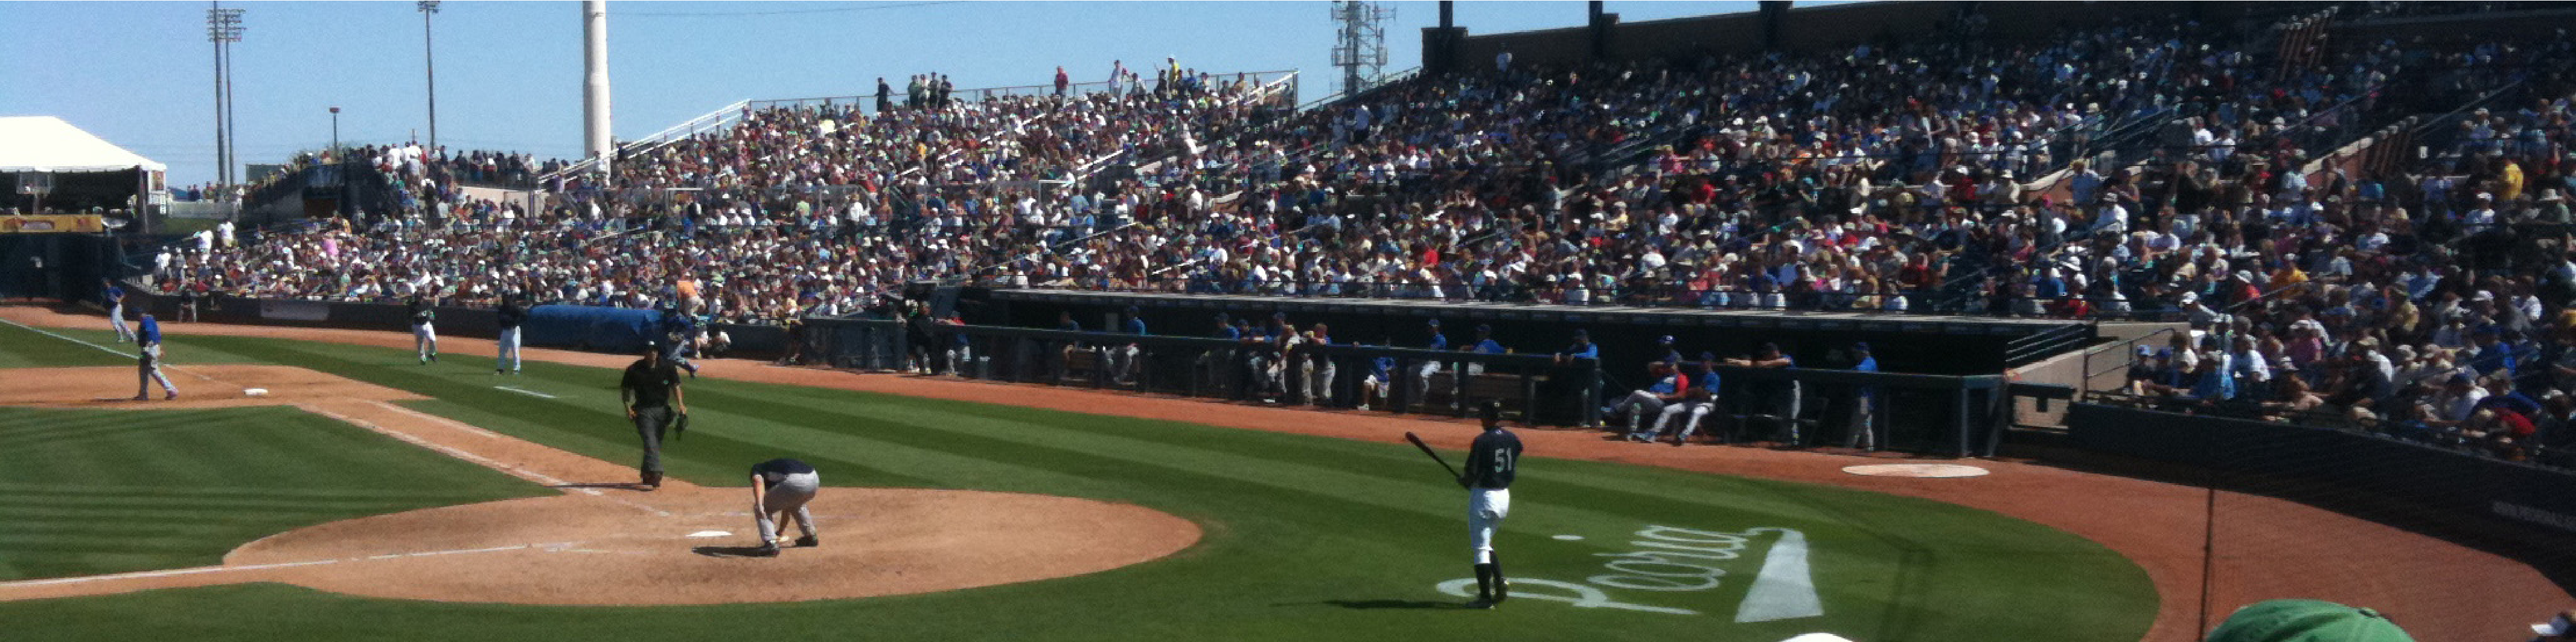
\includegraphics[width=\textwidth]{sampleteaser}
%  \caption{Seattle Mariners at Spring Training, 2010.}
%  \Description{Enjoying the baseball game from the third-base
%  seats. Ichiro Suzuki preparing to bat.}
%  \label{fig:teaser}
%\end{teaserfigure}

%\received{20 February 2007}
%\received[revised]{12 March 2009}
%\received[accepted]{5 June 2009}

\newcommand{\VerbBar}{|}
\newcommand{\VERB}{\Verb[commandchars=\\\{\}]}
\DefineVerbatimEnvironment{Highlighting}{Verbatim}{commandchars=\\\{\}}
\definecolor{shadecolor}{RGB}{248,248,248}
\newenvironment{Shaded}{\begin{snugshade}}{\end{snugshade}}
\newcommand{\AlertTok}[1]{\textcolor[rgb]{1.00,0.00,0.00}{\textbf{#1}}}
\newcommand{\AnnotationTok}[1]{\textcolor[rgb]{0.38,0.63,0.69}{\textbf{\textit{#1}}}}
\newcommand{\AttributeTok}[1]{\textcolor[rgb]{0.49,0.56,0.16}{#1}}
\newcommand{\BaseNTok}[1]{\textcolor[rgb]{0.25,0.63,0.44}{#1}}
\newcommand{\BuiltInTok}[1]{\textcolor[rgb]{0.00,0.50,0.00}{#1}}
\newcommand{\CharTok}[1]{\textcolor[rgb]{0.25,0.44,0.63}{#1}}
\newcommand{\CommentTok}[1]{\textcolor[rgb]{0.38,0.63,0.69}{\textit{#1}}}
\newcommand{\CommentVarTok}[1]{\textcolor[rgb]{0.38,0.63,0.69}{\textbf{\textit{#1}}}}
\newcommand{\ConstantTok}[1]{\textcolor[rgb]{0.53,0.00,0.00}{#1}}
\newcommand{\ControlFlowTok}[1]{\textcolor[rgb]{0.00,0.44,0.13}{\textbf{#1}}}
\newcommand{\DataTypeTok}[1]{\textcolor[rgb]{0.56,0.13,0.00}{#1}}
\newcommand{\DecValTok}[1]{\textcolor[rgb]{0.25,0.63,0.44}{#1}}
\newcommand{\DocumentationTok}[1]{\textcolor[rgb]{0.73,0.13,0.13}{\textit{#1}}}
\newcommand{\ErrorTok}[1]{\textcolor[rgb]{1.00,0.00,0.00}{\textbf{#1}}}
\newcommand{\ExtensionTok}[1]{#1}
\newcommand{\FloatTok}[1]{\textcolor[rgb]{0.25,0.63,0.44}{#1}}
\newcommand{\FunctionTok}[1]{\textcolor[rgb]{0.02,0.16,0.49}{#1}}
\newcommand{\ImportTok}[1]{\textcolor[rgb]{0.00,0.50,0.00}{\textbf{#1}}}
\newcommand{\InformationTok}[1]{\textcolor[rgb]{0.38,0.63,0.69}{\textbf{\textit{#1}}}}
\newcommand{\KeywordTok}[1]{\textcolor[rgb]{0.00,0.44,0.13}{\textbf{#1}}}
\newcommand{\NormalTok}[1]{#1}
\newcommand{\OperatorTok}[1]{\textcolor[rgb]{0.40,0.40,0.40}{#1}}
\newcommand{\OtherTok}[1]{\textcolor[rgb]{0.00,0.44,0.13}{#1}}
\newcommand{\PreprocessorTok}[1]{\textcolor[rgb]{0.74,0.48,0.00}{#1}}
\newcommand{\RegionMarkerTok}[1]{#1}
\newcommand{\SpecialCharTok}[1]{\textcolor[rgb]{0.25,0.44,0.63}{#1}}
\newcommand{\SpecialStringTok}[1]{\textcolor[rgb]{0.73,0.40,0.53}{#1}}
\newcommand{\StringTok}[1]{\textcolor[rgb]{0.25,0.44,0.63}{#1}}
\newcommand{\VariableTok}[1]{\textcolor[rgb]{0.10,0.09,0.49}{#1}}
\newcommand{\VerbatimStringTok}[1]{\textcolor[rgb]{0.25,0.44,0.63}{#1}}
\newcommand{\WarningTok}[1]{\textcolor[rgb]{0.38,0.63,0.69}{\textbf{\textit{#1}}}}

%%
%% This command processes the author and affiliation and title
%% information and builds the first part of the formatted document.
\maketitle

\section{Representing patterns in Functiona Reactive
Programming}\label{representing-patterns-in-functiona-reactive-programming}

Functional Reactive Programming (FRP) was first implemented by Conal
Elliot in Fran {[}1{]}, based on a formal definition of behaviour as a
continuous function of time. Popular implementations of FRP (e.g.~the
Elm language) have followed which have instead opted for discrete rather
than continuous semantics. The following introduces an approach that
supports both discrete and continuous time, developed and popularised
over the past ten years in the TidalCycles system, which is designed for
creative, live exploration of musical (and other) patterns.

In the following I will step us through the process of building a
representation, taking Elliot's definition of behaviour in Fran as a
worthy starting point, and the definition of pattern in TidalCycles as
an end point (with some simplifications). This is done in a practical,
literate programming style, using the Haskell programming language.
Example patterns are visualised, generated directly from the code in
this paper.

Our starting point then, is the \texttt{Behaviour} type from Fran:

\begin{Shaded}
\begin{Highlighting}[]
\KeywordTok{type} \DataTypeTok{Time} \OtherTok{=} \DataTypeTok{Double}
\KeywordTok{type} \DataTypeTok{Behaviour}\NormalTok{ a }\OtherTok{=} \DataTypeTok{Time} \OtherTok{{-}\textgreater{}}\NormalTok{ [a]}
\end{Highlighting}
\end{Shaded}

This represents behaviours elegantly as functions of time, or in other
words, time-varying values. There might be more than one value active at
a particular point in time, hence these behaviours returns a list of
values. Fran also defines an event model, but here we focus entirely on
pure behaviours that have no state beyond time.

\subsection{Rational time}\label{rational-time}

According to Elliot, time in FRP should be \emph{real}, therefore having
arbitrary levels of precision, without building a notion of samplerate
into the representation itself. In practice, Fran uses double-precision
floating point numbers for representing time. Floating point numbers are
certainly efficient, but leave us with the problem of how to deal with
associated errors in time calculations, for instance by building some
tolerance into comparison between values.

To avoid such floating point headaches, here I instead use rational time
as a practical alternative. Unlike floating point numbers, this will
support ratios that are common in media arts, e.g.~durations of 1/3 for
triplets in music, and 1/24 for frame frequencies in video animation.

\begin{Shaded}
\begin{Highlighting}[]
\KeywordTok{type} \DataTypeTok{Time} \OtherTok{=} \DataTypeTok{Rational}
\KeywordTok{type} \DataTypeTok{Pattern}\NormalTok{ a }\OtherTok{=} \DataTypeTok{Time} \OtherTok{{-}\textgreater{}}\NormalTok{ [a]}
\end{Highlighting}
\end{Shaded}

But this raises a question -- what are these numbers a ratio \emph{of}?
The answer is metric cycles, which in music have particular meaning
depending on the musical tradition at play. For example in Western
classical music, metric cycles are referred to as measures or bars, and
in Indian classical music as the nuanced structures of Tala cycles. In
TidalCycles they are simply referred as cycles, and the integer timeline
(i.e., those ratios of \texttt{1}) marks out the endings and beginnings
of successive cycles. For example, a ratio of 4/10 would fall halfway
through the third cycle, counting from zero.

I have also renamed the \texttt{Behaviour} type to \texttt{Pattern} in
the above. This differentiates our type from Elliot's, and connects our
type with the long history of pattern-making.

\subsection{Timespans and events}\label{timespans-and-events}

Next, in order to support discrete events, I introduce time\emph{spans}
to the representation.

\begin{Shaded}
\begin{Highlighting}[]
\KeywordTok{data} \DataTypeTok{TimeSpan} \OtherTok{=} \DataTypeTok{TimeSpan}\NormalTok{ \{}\OtherTok{begin ::} \DataTypeTok{Time}\NormalTok{,}\OtherTok{ end ::} \DataTypeTok{Time}\NormalTok{\}}
\KeywordTok{data} \DataTypeTok{Event}\NormalTok{ a }\OtherTok{=} \DataTypeTok{Event}\NormalTok{ \{}\OtherTok{active ::} \DataTypeTok{TimeSpan}\NormalTok{,}\OtherTok{ value ::}\NormalTok{ a\}}
\KeywordTok{type} \DataTypeTok{Pattern}\NormalTok{ a }\OtherTok{=} \DataTypeTok{TimeSpan} \OtherTok{{-}\textgreater{}}\NormalTok{ [}\DataTypeTok{Event}\NormalTok{ a]}
\end{Highlighting}
\end{Shaded}

A pattern is now a function of timespans to events, and each event is
active for a timespan. A pattern can then be queried with contiguous
timespans, avoiding any chance of missing events that that would fall
between queries of single time values.

However, we also need to take into account that an event might well not
fit within the timespan of a given query. We often need to know
\emph{which} part of an event is active within the queried timespan, and
whether it started before and/or continues beyond that timespan. For
this reason, I add another field to our Event datatype called
\texttt{whole}.

\begin{Shaded}
\begin{Highlighting}[]
\KeywordTok{data} \DataTypeTok{Event}\NormalTok{ a }\OtherTok{=} \DataTypeTok{Event}\NormalTok{ \{}\OtherTok{whole ::} \DataTypeTok{TimeSpan}\NormalTok{,}\OtherTok{ active ::} \DataTypeTok{TimeSpan}\NormalTok{,}\OtherTok{ value ::}\NormalTok{ a\}}
\end{Highlighting}
\end{Shaded}

The `\texttt{whole} timespan of the event must either be the same as or
greater than the \texttt{active} part, and always include it. We use the
\texttt{active} timespan to see when an event is active during the
query, but can compare it with the \texttt{whole} to check whether the
event is a fragment of a larger timespan.

Now the \texttt{Pattern} type can represent discrete events, but it
would be best if it could still represent continuous values.
Fundamentally, a continuous value is one which does not have a discrete
beginning and end. So to represent them, we simply need to make the
`whole' optional, using Haskell's standard \texttt{Maybe} type.

\begin{Shaded}
\begin{Highlighting}[]
\KeywordTok{data} \DataTypeTok{Event}\NormalTok{ a }\OtherTok{=} \DataTypeTok{Event}\NormalTok{ \{}\OtherTok{whole ::} \DataTypeTok{Maybe} \DataTypeTok{TimeSpan}\NormalTok{,}\OtherTok{ active ::} \DataTypeTok{TimeSpan}\NormalTok{,}\OtherTok{ value ::}\NormalTok{ a\}}
\end{Highlighting}
\end{Shaded}

We can now tell when an event is continuous, because its \texttt{whole}
is set to \texttt{Nothing}.

The types are now complete, as follows.

\begin{Shaded}
\begin{Highlighting}[]
\KeywordTok{type} \DataTypeTok{Time} \OtherTok{=} \DataTypeTok{Rational}
\KeywordTok{data} \DataTypeTok{TimeSpan} \OtherTok{=} \DataTypeTok{TimeSpan}\NormalTok{ \{}\OtherTok{begin ::} \DataTypeTok{Time}\NormalTok{,}\OtherTok{ end ::} \DataTypeTok{Time}\NormalTok{\}}
    \KeywordTok{deriving} \DataTypeTok{Show}
\KeywordTok{data} \DataTypeTok{Event}\NormalTok{ a }\OtherTok{=} \DataTypeTok{Event}\NormalTok{ \{}\OtherTok{whole ::} \DataTypeTok{Maybe} \DataTypeTok{TimeSpan}\NormalTok{,}\OtherTok{ active ::} \DataTypeTok{TimeSpan}\NormalTok{,}\OtherTok{ value ::}\NormalTok{ a\}}
    \KeywordTok{deriving}\NormalTok{ (}\DataTypeTok{Show}\NormalTok{, }\DataTypeTok{Functor}\NormalTok{)}
\KeywordTok{data} \DataTypeTok{Pattern}\NormalTok{ a }\OtherTok{=} \DataTypeTok{Pattern}\NormalTok{ \{}\OtherTok{query ::} \DataTypeTok{TimeSpan} \OtherTok{{-}\textgreater{}}\NormalTok{ [}\DataTypeTok{Event}\NormalTok{ a]\}}
    \KeywordTok{deriving}\NormalTok{ (}\DataTypeTok{Functor}\NormalTok{)}
\end{Highlighting}
\end{Shaded}

\section{Constructing patterns}\label{constructing-patterns}

How does this work in practice? Let's have a look at how simple patterns
are defined. For continuous patterns, we simply sample a value at the
halfway point of the queried timespan. For example, a sinewave with a
period of one cycle:

\begin{Shaded}
\begin{Highlighting}[]
\OtherTok{sinewave ::} \DataTypeTok{Pattern} \DataTypeTok{Double}
\NormalTok{sinewave }\OtherTok{=} \DataTypeTok{Pattern} \OperatorTok{$}\NormalTok{ \textbackslash{}timespan }\OtherTok{{-}\textgreater{}}
\NormalTok{  [}\DataTypeTok{Event} \DataTypeTok{Nothing}\NormalTok{ timespan }\OperatorTok{$} \FunctionTok{sin} \OperatorTok{$}\NormalTok{ (}\FunctionTok{fromRational} \OperatorTok{$}\NormalTok{ t timespan) }\OperatorTok{*} \FunctionTok{pi} \OperatorTok{*} \DecValTok{2}\NormalTok{]}
    \KeywordTok{where}\NormalTok{ t timespan }\OtherTok{=}\NormalTok{ begin timespan }\OperatorTok{+}\NormalTok{ ((end timespan }\OperatorTok{{-}}\NormalTok{ begin timespan) }\OperatorTok{/} \DecValTok{2}\NormalTok{)}
\end{Highlighting}
\end{Shaded}

Discrete patterns need to calculate both the whole and active timespans
for each event. The following \texttt{atom} function returns a pattern
that repeats the given value as a discrete event, every cycle. To do
this it splits the query at cycle boundaries, and sets the whole to be
the beginning and end of the cycle for each event. A note on terminology
- in Indian music, the \texttt{sam} is the beginning of a cycle (and end
of the previous one).

\begin{Shaded}
\begin{Highlighting}[]
\NormalTok{sam,}\OtherTok{ nextSam ::} \DataTypeTok{Rational} \OtherTok{{-}\textgreater{}} \DataTypeTok{Rational}
\NormalTok{sam t }\OtherTok{=} \FunctionTok{toRational}\NormalTok{ (}\FunctionTok{floor}\OtherTok{ t ::} \DataTypeTok{Int}\NormalTok{)}
\NormalTok{nextSam }\OtherTok{=}\NormalTok{ (}\DecValTok{1} \OperatorTok{+}\NormalTok{) }\OperatorTok{.}\NormalTok{ sam}

\OtherTok{splitSpan ::} \DataTypeTok{TimeSpan} \OtherTok{{-}\textgreater{}}\NormalTok{ [}\DataTypeTok{TimeSpan}\NormalTok{]}
\NormalTok{splitSpan (}\DataTypeTok{TimeSpan}\NormalTok{ s e) }\OperatorTok{|}\NormalTok{ sam s }\OperatorTok{==}\NormalTok{ sam e }\OperatorTok{||}\NormalTok{ n }\OperatorTok{==}\NormalTok{ e }\OtherTok{=}\NormalTok{ [}\DataTypeTok{TimeSpan}\NormalTok{ s e]}
                         \OperatorTok{|} \FunctionTok{otherwise} \OtherTok{=} \DataTypeTok{TimeSpan}\NormalTok{ s n }\OperatorTok{:}\NormalTok{ splitSpan (}\DataTypeTok{TimeSpan}\NormalTok{ n e)}
    \KeywordTok{where}\NormalTok{ n }\OtherTok{=}\NormalTok{ nextSam s}

\OtherTok{atom ::}\NormalTok{ a }\OtherTok{{-}\textgreater{}} \DataTypeTok{Pattern}\NormalTok{ a}
\NormalTok{atom value }\OtherTok{=} \DataTypeTok{Pattern} \OperatorTok{$} \FunctionTok{map}\NormalTok{ (\textbackslash{}timespan }\OtherTok{{-}\textgreater{}}
                              \DataTypeTok{Event}\NormalTok{ (}\DataTypeTok{Just} \OperatorTok{$} \DataTypeTok{TimeSpan}\NormalTok{ (sam }\OperatorTok{$}\NormalTok{ begin timespan)}
\NormalTok{                                                     (nextSam }\OperatorTok{$}\NormalTok{ begin timespan)}
\NormalTok{                                    )}
\NormalTok{                                    timespan}
\NormalTok{                                    value}
\NormalTok{                           ) }\OperatorTok{.}\NormalTok{ splitSpan}
\end{Highlighting}
\end{Shaded}

\section{Composing patterns}\label{composing-patterns}

Patterns are not too much use until they are composed together, and
because they are functions, we of course need to do functional
composition, by making a new function that calls two or more existing
ones. First, here is a straightforward \texttt{stack} function for
composing patterns together so that they run concurrently:

\begin{Shaded}
\begin{Highlighting}[]
\OtherTok{stack ::}\NormalTok{ [}\DataTypeTok{Pattern}\NormalTok{ a] }\OtherTok{{-}\textgreater{}} \DataTypeTok{Pattern}\NormalTok{ a}
\NormalTok{stack pats }\OtherTok{=} \DataTypeTok{Pattern} \OperatorTok{$}\NormalTok{ \textbackslash{}timespan }\OtherTok{{-}\textgreater{}} \FunctionTok{concatMap}\NormalTok{ (}\OtherTok{\textasciigrave{}query\textasciigrave{}}\NormalTok{ timespan) pats}
\end{Highlighting}
\end{Shaded}

\begin{Shaded}
\begin{Highlighting}[]
\NormalTok{fig1 }\OtherTok{=}\NormalTok{ stack [atom pink, atom purple]}
\end{Highlighting}
\end{Shaded}

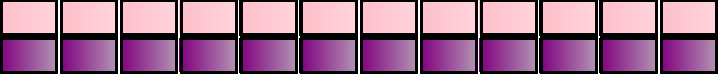
\includegraphics{../figures/fig1.pdf}\\

The above visualises twelve cycles of the pattern over time, from left
to right. Combining patterns in sequence over time is a little
complicated because patterns have infinite length, so we are not able to
simply concatenate them. Instead, we can `interlace' their cycles.

\begin{Shaded}
\begin{Highlighting}[]
\OtherTok{splitQueries ::} \DataTypeTok{Pattern}\NormalTok{ a }\OtherTok{{-}\textgreater{}} \DataTypeTok{Pattern}\NormalTok{ a}
\NormalTok{splitQueries pat }\OtherTok{=}  \DataTypeTok{Pattern} \OperatorTok{$} \FunctionTok{concatMap}\NormalTok{ (query pat) }\OperatorTok{.}\NormalTok{ splitSpan}

\CommentTok{{-}{-} Take a cycle from each pattern in turn}
\OtherTok{interlace ::}\NormalTok{ [}\DataTypeTok{Pattern}\NormalTok{ a] }\OtherTok{{-}\textgreater{}} \DataTypeTok{Pattern}\NormalTok{ a}
\NormalTok{interlace pats }\OtherTok{=}\NormalTok{ splitQueries }\OperatorTok{$} \DataTypeTok{Pattern}\NormalTok{ f}
  \KeywordTok{where}\NormalTok{ f timespan }\OtherTok{=}\NormalTok{ query (\_late offset pat) timespan}
              \KeywordTok{where}\NormalTok{ n }\OtherTok{=} \FunctionTok{toRational} \OperatorTok{$} \FunctionTok{length}\NormalTok{ pats}
\NormalTok{                    cyc }\OtherTok{=}\NormalTok{ sam }\OperatorTok{$}\NormalTok{ begin timespan}
\NormalTok{                    pat }\OtherTok{=}\NormalTok{ pats }\OperatorTok{!!} \FunctionTok{floor}\NormalTok{ (cyc }\OtherTok{\textasciigrave{}mod\textquotesingle{}\textasciigrave{}}\NormalTok{ (}\OtherTok{n ::} \DataTypeTok{Rational}\NormalTok{))}
\NormalTok{                    offset }\OtherTok{=}\NormalTok{ cyc }\OperatorTok{{-}}\NormalTok{ sam (begin timespan }\OperatorTok{/}\NormalTok{ n)}

\CommentTok{{-}{-} The same as interlace, but a cycle from each pattern is taken, interlaced}
\CommentTok{{-}{-} and squashed into a single cycle.}
\OtherTok{interlaceCycle ::}\NormalTok{ [}\DataTypeTok{Pattern}\NormalTok{ a] }\OtherTok{{-}\textgreater{}} \DataTypeTok{Pattern}\NormalTok{ a}
\NormalTok{interlaceCycle pats }\OtherTok{=}\NormalTok{ \_fast (}\FunctionTok{fromIntegral} \OperatorTok{$} \FunctionTok{length}\NormalTok{ pats) }\OperatorTok{$}\NormalTok{ interlace pats}
\end{Highlighting}
\end{Shaded}

Let's look at a visualisation of the first six cycles of a pattern
composed using both \texttt{interlace} and \texttt{stack}. In the
following time is from left to right, with the vertical axis used to
show simultaneously occuring events.

\begin{Shaded}
\begin{Highlighting}[]
\NormalTok{fig2 }\OtherTok{=}\NormalTok{ interlace [atom pink, atom purple]}
\end{Highlighting}
\end{Shaded}


\includegraphics{../figures/fig2.pdf}\\

We can now combine stacks and interlacements:

\begin{Shaded}
\begin{Highlighting}[]
\NormalTok{fig3 }\OtherTok{=}\NormalTok{ stack [atom red,}
\NormalTok{              interlace [atom pink, interlace [atom purple, atom orange]]}
\NormalTok{             ]}
\end{Highlighting}
\end{Shaded}


\includegraphics{../figures/fig3.pdf}\\

\section{Manipulating time}\label{manipulating-time}

A good thing about pure FRP is that it is possible to manipulate time by
making a new function that simply adjusts the time query that is passed
to another function. However our representation has timespans in two
places -- the query and in the events that result. To facilitate the
corrent manipulation of both, I define some utility functions for
working with query and event time:

\begin{Shaded}
\begin{Highlighting}[]
\OtherTok{withSpanTime ::}\NormalTok{ (}\DataTypeTok{Time} \OtherTok{{-}\textgreater{}} \DataTypeTok{Time}\NormalTok{) }\OtherTok{{-}\textgreater{}} \DataTypeTok{TimeSpan} \OtherTok{{-}\textgreater{}} \DataTypeTok{TimeSpan}
\NormalTok{withSpanTime timef (}\DataTypeTok{TimeSpan}\NormalTok{ b e) }\OtherTok{=} \DataTypeTok{TimeSpan}\NormalTok{ (timef b) (timef e)}

\OtherTok{withQueryTime ::}\NormalTok{ (}\DataTypeTok{Time} \OtherTok{{-}\textgreater{}} \DataTypeTok{Time}\NormalTok{) }\OtherTok{{-}\textgreater{}} \DataTypeTok{Pattern}\NormalTok{ a }\OtherTok{{-}\textgreater{}} \DataTypeTok{Pattern}\NormalTok{ a}
\NormalTok{withQueryTime timef (}\DataTypeTok{Pattern}\NormalTok{ q) }\OtherTok{=} \DataTypeTok{Pattern} \OperatorTok{$}\NormalTok{ q }\OperatorTok{.}\NormalTok{ withSpanTime timef}

\OtherTok{withEventTime ::}\NormalTok{ (}\DataTypeTok{Time} \OtherTok{{-}\textgreater{}} \DataTypeTok{Time}\NormalTok{) }\OtherTok{{-}\textgreater{}} \DataTypeTok{Pattern}\NormalTok{ a }\OtherTok{{-}\textgreater{}} \DataTypeTok{Pattern}\NormalTok{ a}
\NormalTok{withEventTime f }\OtherTok{=}\NormalTok{ withEvent }\OperatorTok{$}\NormalTok{ \textbackslash{}e }\OtherTok{{-}\textgreater{}}\NormalTok{ e \{active }\OtherTok{=}\NormalTok{ withSpanTime f }\OperatorTok{$}\NormalTok{ active e,}
\NormalTok{                                       whole }\OtherTok{=}\NormalTok{ withSpanTime f }\OperatorTok{\textless{}$\textgreater{}}\NormalTok{ whole e}
\NormalTok{                                      \}}
    \KeywordTok{where}\NormalTok{ withEvent ef (}\DataTypeTok{Pattern}\NormalTok{ q) }\OtherTok{=} \DataTypeTok{Pattern} \OperatorTok{$} \FunctionTok{map}\NormalTok{ ef }\OperatorTok{\textless{}$\textgreater{}}\NormalTok{ q}

\OtherTok{withTime ::}\NormalTok{ (}\DataTypeTok{Time} \OtherTok{{-}\textgreater{}} \DataTypeTok{Time}\NormalTok{) }\OtherTok{{-}\textgreater{}}\NormalTok{ (}\DataTypeTok{Time} \OtherTok{{-}\textgreater{}} \DataTypeTok{Time}\NormalTok{) }\OtherTok{{-}\textgreater{}} \DataTypeTok{Pattern}\NormalTok{ a }\OtherTok{{-}\textgreater{}} \DataTypeTok{Pattern}\NormalTok{ a}
\NormalTok{withTime fa fb pat }\OtherTok{=}\NormalTok{ withEventTime fa }\OperatorTok{$}\NormalTok{ withQueryTime fb pat}
\end{Highlighting}
\end{Shaded}

It is then straightforward to define functions for making patterned
events to be faster or slower, or shifting them in time to be early or
late. For example to make a pattern `faster', query time is divided and
event time is multiplied by a given factor. This queries a wider window,
and `squashes' the results back into the requested timespan.

\begin{Shaded}
\begin{Highlighting}[]
\NormalTok{\_fast, \_slow, \_late,}\OtherTok{ \_early ::} \DataTypeTok{Time} \OtherTok{{-}\textgreater{}} \DataTypeTok{Pattern}\NormalTok{ a }\OtherTok{{-}\textgreater{}} \DataTypeTok{Pattern}\NormalTok{ a}
\NormalTok{\_fast t  }\OtherTok{=}\NormalTok{ withEventTime (}\OperatorTok{/}\NormalTok{ t) }\OperatorTok{.}\NormalTok{ withQueryTime (}\OperatorTok{*}\NormalTok{ t)}
\NormalTok{\_slow t  }\OtherTok{=}\NormalTok{ withEventTime (}\OperatorTok{*}\NormalTok{ t) }\OperatorTok{.}\NormalTok{ withQueryTime (}\OperatorTok{/}\NormalTok{ t)}
\NormalTok{\_early t }\OtherTok{=}\NormalTok{ withEventTime (}\FunctionTok{subtract}\NormalTok{ t) }\OperatorTok{.}\NormalTok{ withQueryTime (}\OperatorTok{+}\NormalTok{ t)}
\NormalTok{\_late t  }\OtherTok{=}\NormalTok{ withEventTime (}\OperatorTok{+}\NormalTok{ t) }\OperatorTok{.}\NormalTok{ withQueryTime (}\FunctionTok{subtract}\NormalTok{ t)}
\end{Highlighting}
\end{Shaded}

We can apply visualisation in understanding how events can become broken
up. If \texttt{interlace} works cycle-by-cycle, what happens if an event
lasts longer than a cycle?

\begin{Shaded}
\begin{Highlighting}[]
\NormalTok{fig4 }\OtherTok{=}\NormalTok{ interlace [atom red, \_slow }\DecValTok{3} \OperatorTok{$}\NormalTok{ atom green]}
\end{Highlighting}
\end{Shaded}


\includegraphics{../figures/fig4.pdf}\\

The jagged edges indicate where wholes begin before, or end after, the
active event timespans. From the above we can see that each green event
has been broken into parts of one cycle each, and interlaced with the
single-cycle red events.

\subsection{Combining patterns with monadic
binds}\label{combining-patterns-with-monadic-binds}

The above functions are prefixed by \texttt{\_}, because they are
considered internal functions and not part of the end-user interface.
The reason for this is that TidalCycles follows the principle that
\emph{everything} is a pattern. Accordingly, we require functions with
the following time signature, where the time factor is also patterned:

\begin{Shaded}
\begin{Highlighting}[]
\NormalTok{fast, slow, late,}\OtherTok{ early ::} \DataTypeTok{Pattern} \DataTypeTok{Time} \OtherTok{{-}\textgreater{}} \DataTypeTok{Pattern}\NormalTok{ a }\OtherTok{{-}\textgreater{}} \DataTypeTok{Pattern}\NormalTok{ a}
\end{Highlighting}
\end{Shaded}

To implement these functions, we somehow need a way to compose patterns
of time together with the patterns that are having their time structures
manipulated. This is where Haskell's monadic bind
(\texttt{\textgreater{}\textgreater{}=}) comes into view, which does
what we want - it lifts functional arguments into contexts such as
patterns. Our problem is now clarified as one of how to define the
\texttt{Pattern} type as an instance of Haskell's standard Monad
typeclass. In particular, we need to define the bind operator
\texttt{\textgreater{}\textgreater{}=} for patterns, with the type
signature
\texttt{Pattern\ a\ -\textgreater{}\ (a\ -\textgreater{}\ Pattern\ b)\ -\textgreater{}\ Pattern\ b}.
So, what should this bind do?

Certainly, our bind will need to create a new pattern, which as we saw
above, will be a function from timespans to events. This function will
need to be composed of other pattern functions, in particular the
`outer' pattern given as the first argument, and `inner' pattern
resulting from the second argument. The big remaining question is, how
do we deal with the event timespans? The two active timespans are
straightforwardly combined, as the intersection. There is ambiguity,
however, in how the two `whole' timespans should be combined.

\href{}{//}: \textless\textgreater{} The events returned from those
inner pattern queries are then collated and returned, with one caveat --
there is ambiguity about what the resulting event's `whole' timespan
should be. It could from from the `outer' or `inner' pattern, or be the
intersection of the two.

This ambiguity comes down to where the pattern \emph{structure} should
come from - should we preserve the structure of the outer pattern, the
inner pattern, or a combination of the two? In the case of the
\texttt{fast} function (and its \texttt{slow}, \texttt{late} and
\texttt{early} friends), we can say that we will always want to preserve
the structure of the inner patterns - the patterns of values which come
second in the function arguments. This is because we only want to
transform a value pattern using a time pattern, but not otherwise change
the value pattern's structure. (We will see examples of functions that
\emph{do} change the structure of events later.)

The following shows how inner, outer and `mix' binds can be implemented.

TODO - this doesn't work well with outer (?) continuous events

\begin{Shaded}
\begin{Highlighting}[]
\OtherTok{bindWith ::}\NormalTok{ (}\DataTypeTok{Maybe} \DataTypeTok{TimeSpan} \OtherTok{{-}\textgreater{}} \DataTypeTok{Maybe} \DataTypeTok{TimeSpan} \OtherTok{{-}\textgreater{}} \DataTypeTok{Maybe} \DataTypeTok{TimeSpan}\NormalTok{) }\OtherTok{{-}\textgreater{}}
                \DataTypeTok{Pattern}\NormalTok{ a }\OtherTok{{-}\textgreater{}}\NormalTok{ (a }\OtherTok{{-}\textgreater{}} \DataTypeTok{Pattern}\NormalTok{ b) }\OtherTok{{-}\textgreater{}} \DataTypeTok{Pattern}\NormalTok{ b}
\NormalTok{bindWith chooseWhole bv f }\OtherTok{=} \DataTypeTok{Pattern} \OperatorTok{$} \FunctionTok{concatMap}\NormalTok{ match }\OperatorTok{.}\NormalTok{ query bv}
  \KeywordTok{where}\NormalTok{ match e }\OtherTok{=} \FunctionTok{map}\NormalTok{ (withWhole e) }\OperatorTok{$}\NormalTok{ query (f }\OperatorTok{$}\NormalTok{ value e) }\OperatorTok{$}\NormalTok{ active e}
\NormalTok{        withWhole e e\textquotesingle{} }\OtherTok{=}\NormalTok{ e\textquotesingle{} \{whole }\OtherTok{=}\NormalTok{ chooseWhole (whole e) (whole e\textquotesingle{})\}}

\OtherTok{innerBind ::} \DataTypeTok{Pattern}\NormalTok{ a }\OtherTok{{-}\textgreater{}}\NormalTok{ (a }\OtherTok{{-}\textgreater{}} \DataTypeTok{Pattern}\NormalTok{ b) }\OtherTok{{-}\textgreater{}} \DataTypeTok{Pattern}\NormalTok{ b}
\NormalTok{innerBind }\OtherTok{=}\NormalTok{ bindWith (}\FunctionTok{flip} \FunctionTok{const}\NormalTok{)}

\OtherTok{outerBind ::} \DataTypeTok{Pattern}\NormalTok{ a }\OtherTok{{-}\textgreater{}}\NormalTok{ (a }\OtherTok{{-}\textgreater{}} \DataTypeTok{Pattern}\NormalTok{ b) }\OtherTok{{-}\textgreater{}} \DataTypeTok{Pattern}\NormalTok{ b}
\NormalTok{outerBind }\OtherTok{=}\NormalTok{ bindWith }\FunctionTok{const}

\OtherTok{mixBind ::} \DataTypeTok{Pattern}\NormalTok{ a }\OtherTok{{-}\textgreater{}}\NormalTok{ (a }\OtherTok{{-}\textgreater{}} \DataTypeTok{Pattern}\NormalTok{ b) }\OtherTok{{-}\textgreater{}} \DataTypeTok{Pattern}\NormalTok{ b}
\NormalTok{mixBind }\OtherTok{=}\NormalTok{ bindWith (liftA2 intersect)}
\end{Highlighting}
\end{Shaded}

In \texttt{mixBind}, the intersection of the event wholes is taken,
therefore combining the time structures of the two patterns in what we
term a `mix' bind. Alternatively, \texttt{innerBind} uses the time
structure of `whole' timespans from the inner pattern, and
\texttt{outerBind} from the outer pattern. The default bind in the
\texttt{Monad} instance is set as a \texttt{mixBind}. I also define an
\texttt{Applicative} instance based on this bind, with additional
\texttt{\textless{}\textless{}*\textgreater{}} and
\texttt{\textless{}*\textgreater{}\textgreater{}} operators based on
outer and inner binds respectively:

\begin{Shaded}
\begin{Highlighting}[]
\KeywordTok{instance} \DataTypeTok{Monad} \DataTypeTok{Pattern} \KeywordTok{where}
\NormalTok{  (}\OperatorTok{\textgreater{}\textgreater{}=}\NormalTok{) }\OtherTok{=}\NormalTok{ mixBind}

\KeywordTok{instance} \DataTypeTok{Applicative} \DataTypeTok{Pattern} \KeywordTok{where}
  \FunctionTok{pure} \OtherTok{=}\NormalTok{ atom}
\NormalTok{  pf }\OperatorTok{\textless{}*\textgreater{}}\NormalTok{ px }\OtherTok{=}\NormalTok{ pf }\OtherTok{\textasciigrave{}mixBind\textasciigrave{}}\NormalTok{ (}\OperatorTok{\textless{}$\textgreater{}}\NormalTok{ px)}

\CommentTok{{-}{-} (\textless{}\textless{}*\textgreater{}), (\textless{}*\textgreater{}\textgreater{}) :: Pattern (a {-}\textgreater{} b) {-}\textgreater{} Pattern a {-}\textgreater{} Pattern b}
\NormalTok{pf }\OperatorTok{\textless{}\textless{}*\textgreater{}}\NormalTok{ px }\OtherTok{=}\NormalTok{ pf }\OtherTok{\textasciigrave{}outerBind\textasciigrave{}}\NormalTok{ (}\OperatorTok{\textless{}$\textgreater{}}\NormalTok{ px)}
\NormalTok{pf }\OperatorTok{\textless{}*\textgreater{}\textgreater{}}\NormalTok{ px }\OtherTok{=}\NormalTok{ pf }\OtherTok{\textasciigrave{}innerBind\textasciigrave{}}\NormalTok{ (}\OperatorTok{\textless{}$\textgreater{}}\NormalTok{ px)}
\end{Highlighting}
\end{Shaded}

Using this, we can make a function \texttt{patternify\_x} that lifts a
function's first argument into a pattern, using \texttt{innerBind} to
preserve the structure of the second argument. This can then be used to
define our \texttt{fast}, \texttt{slow}, \texttt{late} and
\texttt{early} functions.

\begin{Shaded}
\begin{Highlighting}[]
\OtherTok{patternify\_x ::}\NormalTok{ (a }\OtherTok{{-}\textgreater{}} \DataTypeTok{Pattern}\NormalTok{ b }\OtherTok{{-}\textgreater{}} \DataTypeTok{Pattern}\NormalTok{ c) }\OtherTok{{-}\textgreater{}}
\NormalTok{  (}\DataTypeTok{Pattern}\NormalTok{ a }\OtherTok{{-}\textgreater{}} \DataTypeTok{Pattern}\NormalTok{ b }\OtherTok{{-}\textgreater{}} \DataTypeTok{Pattern}\NormalTok{ c)}
\NormalTok{patternify\_x f ba bb }\OtherTok{=}\NormalTok{ ba }\OtherTok{\textasciigrave{}innerBind\textasciigrave{}}\NormalTok{ \textbackslash{}a }\OtherTok{{-}\textgreater{}}\NormalTok{ f a bb}

\NormalTok{fast, slow, late,}\OtherTok{ early ::} \DataTypeTok{Pattern} \DataTypeTok{Time} \OtherTok{{-}\textgreater{}} \DataTypeTok{Pattern}\NormalTok{ a }\OtherTok{{-}\textgreater{}} \DataTypeTok{Pattern}\NormalTok{ a}
\NormalTok{fast }\OtherTok{=}\NormalTok{ patternify\_x \_fast}
\NormalTok{slow }\OtherTok{=}\NormalTok{ patternify\_x \_slow}
\NormalTok{late }\OtherTok{=}\NormalTok{ patternify\_x \_late}
\NormalTok{early }\OtherTok{=}\NormalTok{ patternify\_x \_early}
\end{Highlighting}
\end{Shaded}

\begin{Shaded}
\begin{Highlighting}[]
\NormalTok{fig5 }\OtherTok{=}\NormalTok{ stack [fast (atom }\FloatTok{1.5}\NormalTok{) p,}
\NormalTok{              slow (atom }\DecValTok{2}\NormalTok{) p}
\NormalTok{             ]}
    \KeywordTok{where}\NormalTok{ p }\OtherTok{=}\NormalTok{ interlace [atom red, atom purple]}
\end{Highlighting}
\end{Shaded}

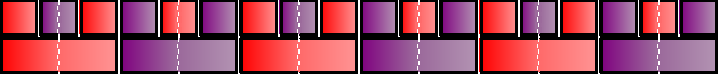
\includegraphics{../figures/fig5.pdf}\\

From the above we can see that the resulting events get split at cycle
boundaries, because the factor patterns (\texttt{atom\ 1.5} and
\texttt{atom\ 2}) repeat every cycle. However more importantly the whole
timespans are preserved, and so the overall time structure is
maintained.\footnote{Note that events are filled with a gradient
  relative to the whole timespans, to visualise which active part of a
  whole timespan each event represents.}

We could avoid this fragmentation by using a continuous rather than a
discrete value in our pattern of factors:

\begin{Shaded}
\begin{Highlighting}[]
\CommentTok{{-}{-} hold a value steady}
\OtherTok{hold ::}\NormalTok{ a }\OtherTok{{-}\textgreater{}} \DataTypeTok{Pattern}\NormalTok{ a}
\NormalTok{hold v }\OtherTok{=} \DataTypeTok{Pattern} \OperatorTok{$}\NormalTok{ \textbackslash{}ts }\OtherTok{{-}\textgreater{}}\NormalTok{ [}\DataTypeTok{Event} \DataTypeTok{Nothing}\NormalTok{ ts v]}

\NormalTok{fig5b }\OtherTok{=}\NormalTok{ stack [fast (hold }\FloatTok{1.5}\NormalTok{) p,}
\NormalTok{               slow (hold }\DecValTok{2}\NormalTok{) p}
\NormalTok{              ]}
    \KeywordTok{where}\NormalTok{ p }\OtherTok{=}\NormalTok{ interlace [atom red, atom purple]}
\end{Highlighting}
\end{Shaded}


\includegraphics{../figures/fig5b.pdf}\\

In practice we can consider the patterns to be equivalent -- the overall
structure is the same, whether or not contituent events have become
fragmented by transformations.

\section{Masking and restructuring
patterns}\label{masking-and-restructuring-patterns}

So far we have looked at the results of inner binds, where the structure
of a transformed pattern is preserved. Lets now compare the use of inner
and outer binds, and in particular their use in masking or restructuring
pattern.

\begin{Shaded}
\begin{Highlighting}[]
\OtherTok{silence ::} \DataTypeTok{Pattern}\NormalTok{ a}
\NormalTok{silence }\OtherTok{=} \DataTypeTok{Pattern} \OperatorTok{$} \FunctionTok{const}\NormalTok{ []}

\OtherTok{\_ifpat ::} \DataTypeTok{Bool} \OtherTok{{-}\textgreater{}} \DataTypeTok{Pattern}\NormalTok{ a }\OtherTok{{-}\textgreater{}} \DataTypeTok{Pattern}\NormalTok{ a}
\NormalTok{\_ifpat }\DataTypeTok{True}\NormalTok{ p }\OtherTok{=}\NormalTok{ p}
\NormalTok{\_ifpat }\DataTypeTok{False}\NormalTok{ \_ }\OtherTok{=}\NormalTok{ silence}

\OtherTok{mask ::} \DataTypeTok{Pattern} \DataTypeTok{Bool} \OtherTok{{-}\textgreater{}} \DataTypeTok{Pattern}\NormalTok{ a }\OtherTok{{-}\textgreater{}} \DataTypeTok{Pattern}\NormalTok{ a}
\NormalTok{mask bp p }\OtherTok{=}\NormalTok{ bp }\OtherTok{\textasciigrave{}innerBind\textasciigrave{}}\NormalTok{ \textbackslash{}b }\OtherTok{{-}\textgreater{}}\NormalTok{ \_ifpat b p}

\OtherTok{struct ::} \DataTypeTok{Pattern} \DataTypeTok{Bool} \OtherTok{{-}\textgreater{}} \DataTypeTok{Pattern}\NormalTok{ a }\OtherTok{{-}\textgreater{}} \DataTypeTok{Pattern}\NormalTok{ a}
\NormalTok{struct bp p }\OtherTok{=}\NormalTok{ bp }\OtherTok{\textasciigrave{}outerBind\textasciigrave{}}\NormalTok{ \textbackslash{}b }\OtherTok{{-}\textgreater{}}\NormalTok{ \_ifpat b p}
\end{Highlighting}
\end{Shaded}

The bind is the only difference between these two functions, but they
have very different practical uses. \texttt{struct} is used to impose a
new structure on a pattern, where as \texttt{mask} maintains the
structure, but masks off some parts of it.

\begin{Shaded}
\begin{Highlighting}[]
\NormalTok{fig6 }\OtherTok{=}\NormalTok{ stack [}
\NormalTok{    pat,}
\NormalTok{    struct (interlaceCycle [atom }\DataTypeTok{True}\NormalTok{, atom }\DataTypeTok{True}\NormalTok{, atom }\DataTypeTok{False}\NormalTok{, atom }\DataTypeTok{True}\NormalTok{]) pat,}
\NormalTok{    mask (interlaceCycle [atom }\DataTypeTok{True}\NormalTok{, atom }\DataTypeTok{True}\NormalTok{, atom }\DataTypeTok{False}\NormalTok{, atom }\DataTypeTok{True}\NormalTok{]) pat}
\NormalTok{  ]}
  \KeywordTok{where}\NormalTok{ pat }\OtherTok{=}\NormalTok{ interlaceCycle [atom red, atom purple]}
\end{Highlighting}
\end{Shaded}

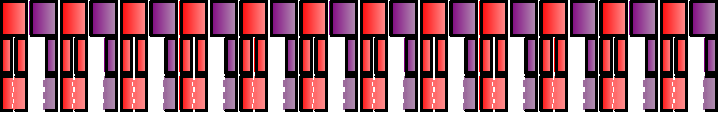
\includegraphics{../figures/fig6.pdf}\\

\section{Combining continuous and discrete
events}\label{combining-continuous-and-discrete-events}

A practical advantage of representing both continuous and discrete
events in one type, is that they can be composed together. For example
the following blends between two different discrete patterns, using a
continuous sinewave:

\begin{Shaded}
\begin{Highlighting}[]
\NormalTok{fig7 }\OtherTok{=}\NormalTok{ atom red }\OtherTok{\textasciigrave{}outerBind\textasciigrave{}}\NormalTok{ \textbackslash{}a}
         \OtherTok{{-}\textgreater{}}\NormalTok{ atom blue }\OtherTok{\textasciigrave{}outerBind\textasciigrave{}}\NormalTok{ \textbackslash{}b}
         \OtherTok{{-}\textgreater{}}\NormalTok{ \_slow }\DecValTok{12}\NormalTok{ sinewave }\OtherTok{\textasciigrave{}outerBind\textasciigrave{}}\NormalTok{ \textbackslash{}x}
         \OtherTok{{-}\textgreater{}} \FunctionTok{return} \OperatorTok{$}\NormalTok{ blend ((x}\OperatorTok{+}\DecValTok{1}\NormalTok{)}\OperatorTok{/}\DecValTok{2}\NormalTok{) a b}
\end{Highlighting}
\end{Shaded}

With the use of \texttt{outerBind}, the structure is taken from the
first pattern, and so the events are discrete.


\includegraphics{../figures/fig7.pdf}\\

Unfortunately, our Pattern monad is not fully lawful, in that flipping
the order of the patterns while also flipping from outer to inner bind,
does not produce the same results as you might hope:

\begin{Shaded}
\begin{Highlighting}[]
\NormalTok{fig8 }\OtherTok{=}\NormalTok{ \_slow }\DecValTok{12}\NormalTok{ sinewave }\OtherTok{\textasciigrave{}innerBind\textasciigrave{}}\NormalTok{ \textbackslash{}x}
         \OtherTok{{-}\textgreater{}}\NormalTok{ atom blue }\OtherTok{\textasciigrave{}innerBind\textasciigrave{}}\NormalTok{ \textbackslash{}b}
         \OtherTok{{-}\textgreater{}}\NormalTok{ atom red }\OtherTok{\textasciigrave{}innerBind\textasciigrave{}}\NormalTok{ \textbackslash{}a}
         \OtherTok{{-}\textgreater{}} \FunctionTok{return} \OperatorTok{$}\NormalTok{ blend ((x}\OperatorTok{+}\DecValTok{1}\NormalTok{)}\OperatorTok{/}\DecValTok{2}\NormalTok{) a b}
\end{Highlighting}
\end{Shaded}


\includegraphics{../figures/fig8.pdf}\\

The reason for this is that to produce the above visualisation, the
resulting pattern is queried for twelve cycles at once. This is passed
to the continuous pattern, which then produces a single event at that
resolution. All is not lost, however, if we combine this resulting
pattern with another discrete one, the correct result is shown again:

\begin{Shaded}
\begin{Highlighting}[]
\NormalTok{fig9 }\OtherTok{=}\NormalTok{ struct (atom }\DataTypeTok{True}\NormalTok{) }\OperatorTok{$}
\NormalTok{        \_slow }\DecValTok{12}\NormalTok{ sinewave }\OtherTok{\textasciigrave{}innerBind\textasciigrave{}}\NormalTok{ \textbackslash{}x}
         \OtherTok{{-}\textgreater{}}\NormalTok{ atom blue }\OtherTok{\textasciigrave{}innerBind\textasciigrave{}}\NormalTok{ \textbackslash{}b}
         \OtherTok{{-}\textgreater{}}\NormalTok{ atom red }\OtherTok{\textasciigrave{}innerBind\textasciigrave{}}\NormalTok{ \textbackslash{}a}
         \OtherTok{{-}\textgreater{}} \FunctionTok{return} \OperatorTok{$}\NormalTok{ blend ((x}\OperatorTok{+}\DecValTok{1}\NormalTok{)}\OperatorTok{/}\DecValTok{2}\NormalTok{) a b}
\end{Highlighting}
\end{Shaded}


\includegraphics{../figures/fig9.pdf}\\

The easiest workaround for this issue is to take care that continuous
patterns are contained within discrete ones. In practice, this can be
taken care of in the design of the combinator library, and is not
something that the end-user programmer needs to worry about.

\appendix

\section{Preamble and supporting
functions}\label{preamble-and-supporting-functions}

\begin{Shaded}
\begin{Highlighting}[]
\KeywordTok{module} \DataTypeTok{Pattern} \KeywordTok{where}

\KeywordTok{import} \DataTypeTok{Control.Applicative}
\KeywordTok{import} \DataTypeTok{Data.Fixed}
\KeywordTok{import} \DataTypeTok{Data.Colour}
\KeywordTok{import} \DataTypeTok{Data.Colour.Names}

\OtherTok{intersect ::} \DataTypeTok{TimeSpan} \OtherTok{{-}\textgreater{}} \DataTypeTok{TimeSpan} \OtherTok{{-}\textgreater{}} \DataTypeTok{TimeSpan}
\NormalTok{intersect (}\DataTypeTok{TimeSpan}\NormalTok{ b e) (}\DataTypeTok{TimeSpan}\NormalTok{ b\textquotesingle{} e\textquotesingle{}) }\OtherTok{=} \DataTypeTok{TimeSpan}\NormalTok{ (}\FunctionTok{max}\NormalTok{ b b\textquotesingle{}) (}\FunctionTok{min}\NormalTok{ e e\textquotesingle{})}
\KeywordTok{infixl} \DecValTok{4} \OperatorTok{\textless{}\textless{}*\textgreater{}}\NormalTok{, }\OperatorTok{\textless{}*\textgreater{}\textgreater{}}
\end{Highlighting}
\end{Shaded}

\section*{References}\label{references}
\addcontentsline{toc}{section}{References}

\phantomsection\label{refs}
\begin{CSLReferences}{0}{0}
\bibitem[\citeproctext]{ref-elliottFunctionalReactiveAnimation1997}
\CSLLeftMargin{{[}1{]} }%
\CSLRightInline{Elliott, C. and Hudak, P. 1997.
\href{https://doi.org/10.1145/258948.258973}{Functional reactive
animation}. \emph{Proceedings of the second ACM SIGPLAN international
conference on Functional programming} (New York, NY, USA, Aug. 1997),
263--273.}

\end{CSLReferences}


\end{document}
\endinput
%%
%% End of file `sample-acmsmall-conf.tex'.
